\begin{examplebox}
\begin{minipage}{\linewidth}
\textbf{\textcolor{CExample}{例 1（基础）}}

	\textbf{\textcolor{CExample}{题目：}}
	求函数 $f(x) = x^5 + 2^x + \log_3 x + \sin x$（$x>0$）的导数.
% F049: native TikZ/PGFPlots, computed from the stated mathematical model.
\begin{center}
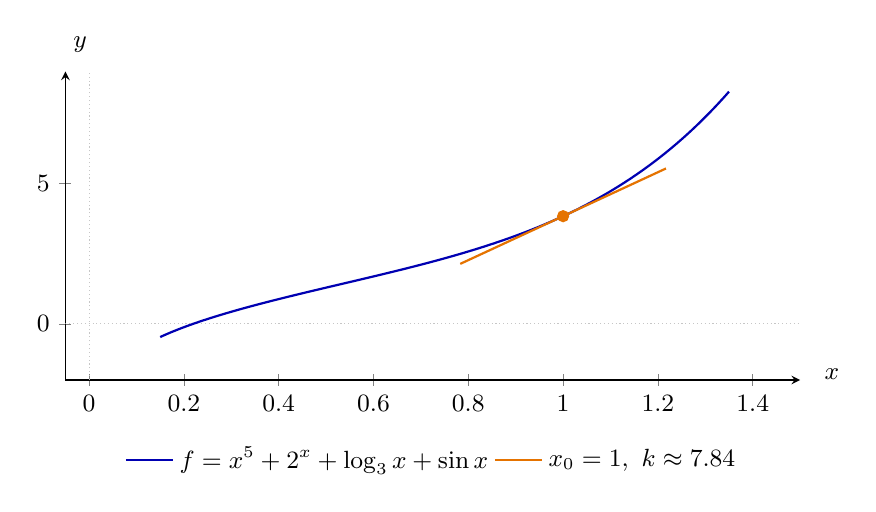
\begin{tikzpicture}[font=\small,>=stealth]
\begin{axis}[width=.90\linewidth,height=5.5cm,xmin=-0.05,xmax=1.5,ymin=-2,ymax=9,
axis lines=left,xlabel={$x$},ylabel={$y$},font=\small,
xlabel style={at={(axis description cs:1.02,.02)},anchor=west},
ylabel style={rotate=-90,at={(axis description cs:.02,1.03)},anchor=south},
legend style={at={(axis description cs:.5,-.18)},anchor=north,draw=none,fill=none,font=\small,legend columns=2},
unbounded coords=jump,clip=true,]
\addplot[gray!45,thin,densely dotted,forget plot] coordinates {(-0.05,0) (1.5,0)};
\addplot[gray!45,thin,densely dotted,forget plot] coordinates {(0,-2) (0,9)};
\addplot[blue!70!black,thick] coordinates {(0.15,-0.46774949) (0.15666667,-0.41642159) (0.16333333,-0.36672313) (0.17,-0.31852181) (0.17666667,-0.27170052) (0.18333333,-0.2261551) (0.19,-0.18179247) (0.19666667,-0.13852911) (0.20333333,-0.096289741) (0.21,-0.055006306) (0.21666667,-0.01461701) (0.22333333,0.024934416) (0.23,0.063699389) (0.23666667,0.10172502) (0.24333333,0.13905463) (0.25,0.17572813) (0.25666667,0.21178241) (0.26333333,0.24725165) (0.27,0.28216761) (0.27666667,0.31655985) (0.28333333,0.35045598) (0.29,0.38388182) (0.29666667,0.41686158) (0.30333333,0.44941802) (0.31,0.48157256) (0.31666667,0.51334544) (0.32333333,0.54475578) (0.33,0.57582173) (0.33666667,0.60656051) (0.34333333,0.6369885) (0.35,0.66712134) (0.35666667,0.69697398) (0.36333333,0.7265607) (0.37,0.75589524) (0.37666667,0.78499078) (0.38333333,0.81386001) (0.39,0.84251521) (0.39666667,0.87096821) (0.40333333,0.89923049) (0.41,0.92731318) (0.41666667,0.95522711) (0.42333333,0.98298281) (0.43,1.0105906) (0.43666667,1.0380604) (0.44333333,1.0654022) (0.45,1.0926256) (0.45666667,1.11974) (0.46333333,1.1467548) (0.47,1.1736791) (0.47666667,1.200522) (0.48333333,1.2272924) (0.49,1.2539992) (0.49666667,1.2806512) (0.50333333,1.307257) (0.51,1.3338253) (0.51666667,1.3603647) (0.52333333,1.3868838) (0.53,1.413391) (0.53666667,1.4398949) (0.54333333,1.4664039) (0.55,1.4929267) (0.55666667,1.5194716) (0.56333333,1.5460472) (0.57,1.5726621) (0.57666667,1.5993248) (0.58333333,1.626044) (0.59,1.6528282) (0.59666667,1.6796861) (0.60333333,1.7066266) (0.61,1.7336584) (0.61666667,1.7607904) (0.62333333,1.7880314) (0.63,1.8153906) (0.63666667,1.842877) (0.64333333,1.8704998) (0.65,1.8982682) (0.65666667,1.9261915) (0.66333333,1.9542793) (0.67,1.9825411) (0.67666667,2.0109864) (0.68333333,2.0396252) (0.69,2.0684671) (0.69666667,2.0975223) (0.70333333,2.1268007) (0.71,2.1563127) (0.71666667,2.1860685) (0.72333333,2.2160787) (0.73,2.2463538) (0.73666667,2.2769046) (0.74333333,2.3077419) (0.75,2.3388768) (0.75666667,2.3703203) (0.76333333,2.4020839) (0.77,2.434179) (0.77666667,2.4666171) (0.78333333,2.49941) (0.79,2.5325697) (0.79666667,2.5661081) (0.80333333,2.6000376) (0.81,2.6343705) (0.81666667,2.6691194) (0.82333333,2.704297) (0.83,2.7399163) (0.83666667,2.7759903) (0.84333333,2.8125322) (0.85,2.8495555) (0.85666667,2.8870739) (0.86333333,2.925101) (0.87,2.963651) (0.87666667,3.0027379) (0.88333333,3.0423761) (0.89,3.0825802) (0.89666667,3.1233649) (0.90333333,3.1647451) (0.91,3.2067361) (0.91666667,3.2493531) (0.92333333,3.2926117) (0.93,3.3365276) (0.93666667,3.3811168) (0.94333333,3.4263955) (0.95,3.4723799) (0.95666667,3.5190868) (0.96333333,3.5665329) (0.97,3.6147352) (0.97666667,3.6637109) (0.98333333,3.7134776) (0.99,3.7640528) (0.99666667,3.8154545) (1.0033333,3.8677009) (1.01,3.9208102) (1.0166667,3.974801) (1.0233333,4.0296923) (1.03,4.0855029) (1.0366667,4.1422522) (1.0433333,4.1999598) (1.05,4.2586454) (1.0566667,4.3183289) (1.0633333,4.3790307) (1.07,4.4407712) (1.0766667,4.5035711) (1.0833333,4.5674515) (1.09,4.6324336) (1.0966667,4.6985388) (1.1033333,4.7657889) (1.11,4.8342059) (1.1166667,4.903812) (1.1233333,4.9746298) (1.13,5.0466821) (1.1366667,5.1199917) (1.1433333,5.1945821) (1.15,5.2704769) (1.1566667,5.3476997) (1.1633333,5.4262749) (1.17,5.5062266) (1.1766667,5.5875795) (1.1833333,5.6703587) (1.19,5.7545892) (1.1966667,5.8402965) (1.2033333,5.9275064) (1.21,6.016245) (1.2166667,6.1065384) (1.2233333,6.1984134) (1.23,6.2918968) (1.2366667,6.3870158) (1.2433333,6.4837978) (1.25,6.5822707) (1.2566667,6.6824624) (1.2633333,6.7844013) (1.27,6.888116) (1.2766667,6.9936355) (1.2833333,7.100989) (1.29,7.2102061) (1.2966667,7.3213166) (1.3033333,7.4343506) (1.31,7.5493386) (1.3166667,7.6663114) (1.3233333,7.7853) (1.33,7.9063358) (1.3366667,8.0294505) (1.3433333,8.1546761) (1.35,8.282045)};
\addlegendentry{$f=x^5+2^x+\log_3x+\sin x$}
\addplot[orange!90!black,thick] coordinates {(0.783,2.1408776) (1.217,5.5420644)};
\addlegendentry{$x_0=1,\ k\approx7.84$}
\addplot[only marks,mark=*,orange!90!black,forget plot] coordinates {(1,3.841471)};

\end{axis}
\end{tikzpicture}
\par\smallskip{\small 按本题原函数绘图；切线斜率由本题的导函数计算。}
\end{center}


\end{minipage}

	\textbf{\textcolor{CExample}{解题步骤：}}
	\begin{description}[style=nextline, leftmargin=2.8em, labelsep=0.5em, itemsep=0.45em]
		\item[\textbf{第一步（识别类型）：}] 将 $f(x)$ 拆分为四项：幂函数 $x^5$，指数函数 $2^x$，对数函数 $\log_3 x$，正弦函数 $\sin x$.
			\par\textbf{理由：} 根据导数的线性性质，和差可以逐项求导.

		\item[\textbf{第二步（逐项求导）：}] 对每一项应用基本导数公式：
			\[
				\begin{aligned}
					(x^5)' &= 5x^{4}, \\
					(2^x)' &= 2^x \ln 2, \\
					(\log_3 x)' &= \frac{1}{x\ln 3}, \\
					(\sin x)' &= \cos x.
			\end{aligned}
			\]
			\par\textbf{理由：} 直接套用幂函数、指数函数、对数函数、正弦函数的导数公式.

		\item[\textbf{第三步（组合结果）：}] 将各项导数相加，得到导函数：
			\[
				f'(x) = 5x^4 + 2^x \ln 2 + \frac{1}{x\ln 3} + \cos x.
			\]
			\par\textbf{理由：} 导数的线性组合性质.
	\end{description}

	\textbf{\textcolor{CExample}{关键结论：}}
	对于基本初等函数的线性组合，只需分别求导后相加即可.

	\medskip
\end{examplebox}

\begin{examplebox}
\begin{minipage}{\linewidth}
\textbf{\textcolor{CExample}{例 2（稍变形）}}

	\textbf{\textcolor{CExample}{题目：}}
	求函数 $g(x) = 5e^x - 4\ln x + 3\cos x$（$x>0$）的导数.
% F049: native TikZ/PGFPlots, computed from the stated mathematical model.
\begin{center}
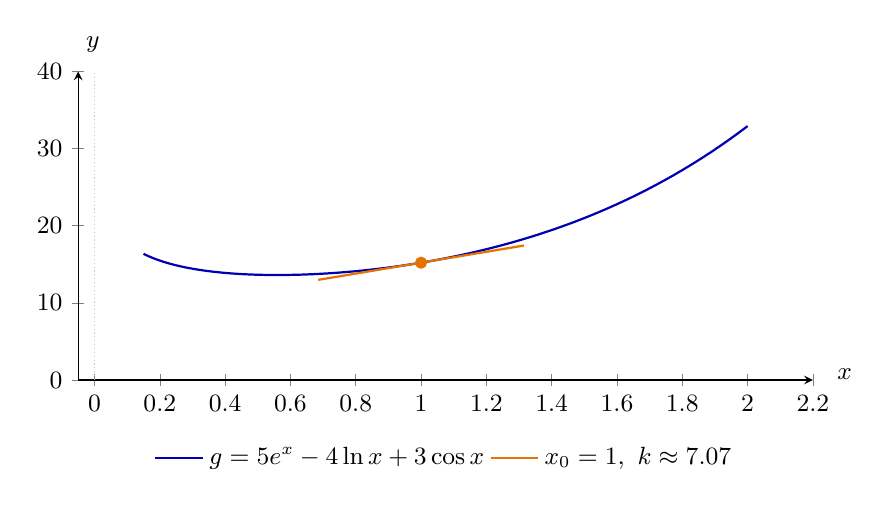
\begin{tikzpicture}[font=\small,>=stealth]
\begin{axis}[width=.90\linewidth,height=5.5cm,xmin=-0.05,xmax=2.2,ymin=0,ymax=40,
axis lines=left,xlabel={$x$},ylabel={$y$},font=\small,
xlabel style={at={(axis description cs:1.02,.02)},anchor=west},
ylabel style={rotate=-90,at={(axis description cs:.02,1.03)},anchor=south},
legend style={at={(axis description cs:.5,-.18)},anchor=north,draw=none,fill=none,font=\small,legend columns=2},
unbounded coords=jump,clip=true,]
\addplot[gray!45,thin,densely dotted,forget plot] coordinates {(0,0) (0,40)};
\addplot[blue!70!black,thick] coordinates {(0.15,16.363964) (0.16027778,16.154121) (0.17055556,15.961066) (0.18083333,15.782878) (0.19111111,15.617952) (0.20138889,15.464941) (0.21166667,15.322696) (0.22194444,15.190237) (0.23222222,15.066714) (0.2425,14.951393) (0.25277778,14.843628) (0.26305556,14.742855) (0.27333333,14.648574) (0.28361111,14.560341) (0.29388889,14.477762) (0.30416667,14.400483) (0.31444444,14.328188) (0.32472222,14.26059) (0.335,14.197432) (0.34527778,14.13848) (0.35555556,14.083521) (0.36583333,14.032362) (0.37611111,13.984828) (0.38638889,13.940756) (0.39666667,13.899999) (0.40694444,13.862421) (0.41722222,13.827898) (0.4275,13.796315) (0.43777778,13.767566) (0.44805556,13.741554) (0.45833333,13.718188) (0.46861111,13.697385) (0.47888889,13.679068) (0.48916667,13.663165) (0.49944444,13.64961) (0.50972222,13.638341) (0.52,13.629302) (0.53027778,13.622439) (0.54055556,13.617703) (0.55083333,13.615048) (0.56111111,13.614432) (0.57138889,13.615816) (0.58166667,13.619163) (0.59194444,13.62444) (0.60222222,13.631614) (0.6125,13.640656) (0.62277778,13.651541) (0.63305556,13.664242) (0.64333333,13.678736) (0.65361111,13.695003) (0.66388889,13.713024) (0.67416667,13.732779) (0.68444444,13.754253) (0.69472222,13.77743) (0.705,13.802298) (0.71527778,13.828843) (0.72555556,13.857056) (0.73583333,13.886925) (0.74611111,13.918442) (0.75638889,13.951599) (0.76666667,13.986389) (0.77694444,14.022807) (0.78722222,14.060848) (0.7975,14.100508) (0.80777778,14.141783) (0.81805556,14.184671) (0.82833333,14.229171) (0.83861111,14.275282) (0.84888889,14.323004) (0.85916667,14.372337) (0.86944444,14.423282) (0.87972222,14.475842) (0.89,14.53002) (0.90027778,14.585817) (0.91055556,14.643238) (0.92083333,14.702287) (0.93111111,14.76297) (0.94138889,14.82529) (0.95166667,14.889255) (0.96194444,14.954871) (0.97222222,15.022144) (0.9825,15.091082) (0.99277778,15.161693) (1.0030556,15.233984) (1.0133333,15.307966) (1.0236111,15.383646) (1.0338889,15.461034) (1.0441667,15.540141) (1.0544444,15.620977) (1.0647222,15.703552) (1.075,15.787879) (1.0852778,15.873967) (1.0955556,15.96183) (1.1058333,16.05148) (1.1161111,16.142929) (1.1263889,16.236191) (1.1366667,16.331279) (1.1469444,16.428206) (1.1572222,16.526987) (1.1675,16.627637) (1.1777778,16.730169) (1.1880556,16.8346) (1.1983333,16.940945) (1.2086111,17.049219) (1.2188889,17.15944) (1.2291667,17.271622) (1.2394444,17.385783) (1.2497222,17.50194) (1.26,17.620111) (1.2702778,17.740313) (1.2805556,17.862565) (1.2908333,17.986884) (1.3011111,18.113289) (1.3113889,18.2418) (1.3216667,18.372436) (1.3319444,18.505215) (1.3422222,18.640159) (1.3525,18.777287) (1.3627778,18.91662) (1.3730556,19.058178) (1.3833333,19.201984) (1.3936111,19.348057) (1.4038889,19.49642) (1.4141667,19.647096) (1.4244444,19.800105) (1.4347222,19.955472) (1.445,20.113218) (1.4552778,20.273367) (1.4655556,20.435943) (1.4758333,20.600969) (1.4861111,20.76847) (1.4963889,20.938469) (1.5066667,21.110992) (1.5169444,21.286064) (1.5272222,21.463711) (1.5375,21.643956) (1.5477778,21.826828) (1.5580556,22.012352) (1.5683333,22.200554) (1.5786111,22.391462) (1.5888889,22.585102) (1.5991667,22.781503) (1.6094444,22.980692) (1.6197222,23.182697) (1.63,23.387546) (1.6402778,23.595269) (1.6505556,23.805895) (1.6608333,24.019453) (1.6711111,24.235973) (1.6813889,24.455484) (1.6916667,24.678018) (1.7019444,24.903605) (1.7122222,25.132276) (1.7225,25.364062) (1.7327778,25.598996) (1.7430556,25.837109) (1.7533333,26.078433) (1.7636111,26.323003) (1.7738889,26.57085) (1.7841667,26.822008) (1.7944444,27.076511) (1.8047222,27.334392) (1.815,27.595688) (1.8252778,27.860432) (1.8355556,28.128659) (1.8458333,28.400406) (1.8561111,28.675708) (1.8663889,28.954601) (1.8766667,29.237123) (1.8869444,29.52331) (1.8972222,29.813199) (1.9075,30.106829) (1.9177778,30.404238) (1.9280556,30.705463) (1.9383333,31.010546) (1.9486111,31.319523) (1.9588889,31.632436) (1.9691667,31.949325) (1.9794444,32.27023) (1.9897222,32.595191) (2,32.924251)};
\addlegendentry{$g=5e^x-4\ln x+3\cos x$}
\addplot[orange!90!black,thick] coordinates {(0.685,12.986212) (1.315,17.43842)};
\addlegendentry{$x_0=1,\ k\approx7.07$}
\addplot[only marks,mark=*,orange!90!black,forget plot] coordinates {(1,15.212316)};

\end{axis}
\end{tikzpicture}
\par\smallskip{\small 按本题原函数绘图；切线斜率由本题的导函数计算。}
\end{center}


\end{minipage}

	\textbf{\textcolor{CExample}{解题步骤：}}
	\begin{description}[style=nextline, leftmargin=2.8em, labelsep=0.5em, itemsep=0.45em]
		\item[\textbf{第一步（识别类型）：}] $g(x)$ 由常数倍 $5e^x$、$-4\ln x$、$3\cos x$ 组成.
			\par\textbf{理由：} 线性性质允许分别处理.

		\item[\textbf{第二步（逐项求导）：}]
			\[
				\begin{aligned}
					(5e^x)' &= 5e^x, \\
					(-4\ln x)' &= -4\cdot\frac{1}{x} \\
					&= -\frac{4}{x}, \\
					(3\cos x)' &= 3(-\sin x) \\
					&= -3\sin x.
			\end{aligned}
			\]
			\par\textbf{理由：} 常数因子可以提到求导符号外面；应用 $e^x$、$\ln x$、$\cos x$ 的导数公式.

		\item[\textbf{第三步（组合结果）：}]
			\[
				g'(x) = 5e^x - \frac{4}{x} - 3\sin x.
			\]
			\par\textbf{理由：} 线性组合相加.
	\end{description}

	\textbf{\textcolor{CExample}{关键结论：}}
	常数因子直接保留；自然对数的导数为 $1/x$，所以 $-4\ln x$ 的导数为 $-4/x$.

	\medskip
\end{examplebox}

\begin{examplebox}
\begin{minipage}{\linewidth}
\textbf{\textcolor{CExample}{例 3（综合应用）}}

	\textbf{\textcolor{CExample}{题目：}}
	求曲线 $y = x^3 + \ln x$ 在点 $(1,1)$ 处的切线方程.
% F049: native TikZ/PGFPlots, computed from the stated mathematical model.
\begin{center}
\begin{tikzpicture}[font=\small,>=stealth]
\begin{axis}[width=.90\linewidth,height=5.5cm,xmin=-0.1,xmax=2,ymin=-3,ymax=8,
axis lines=left,xlabel={$x$},ylabel={$y$},font=\small,
xlabel style={at={(axis description cs:1.02,.02)},anchor=west},
ylabel style={rotate=-90,at={(axis description cs:.02,1.03)},anchor=south},
legend style={at={(axis description cs:.5,-.18)},anchor=north,draw=none,fill=none,font=\small,legend columns=2},
unbounded coords=jump,clip=true,]
\addplot[gray!45,thin,densely dotted,forget plot] coordinates {(-0.1,0) (2,0)};
\addplot[gray!45,thin,densely dotted,forget plot] coordinates {(0,-3) (0,8)};
\addplot[blue!70!black,thick] coordinates {(0.18,-1.7089664) (0.189,-1.659257) (0.198,-1.6117259) (0.207,-1.5661667) (0.216,-1.5223992) (0.225,-1.4802643) (0.234,-1.4396213) (0.243,-1.4003449) (0.252,-1.3623232) (0.261,-1.3254553) (0.27,-1.2896503) (0.279,-1.2548259) (0.288,-1.2209069) (0.297,-1.1878251) (0.306,-1.1555176) (0.315,-1.1239268) (0.324,-1.0929995) (0.333,-1.0626868) (0.342,-1.0329429) (0.351,-1.0037255) (0.36,-0.97499525) (0.369,-0.94671523) (0.378,-0.91885093) (0.387,-0.89136998) (0.396,-0.86424193) (0.405,-0.83743809) (0.414,-0.81093136) (0.423,-0.78469613) (0.432,-0.75870812) (0.441,-0.73294428) (0.45,-0.7073827) (0.459,-0.68200249) (0.468,-0.65678375) (0.477,-0.63170746) (0.486,-0.6067554) (0.495,-0.58191014) (0.504,-0.55715495) (0.513,-0.53247374) (0.522,-0.50785104) (0.531,-0.48327197) (0.54,-0.45872214) (0.549,-0.43418769) (0.558,-0.4096552) (0.567,-0.38511171) (0.576,-0.36054464) (0.585,-0.33594181) (0.594,-0.31129138) (0.603,-0.28658186) (0.612,-0.26180207) (0.621,-0.23694114) (0.63,-0.21198846) (0.639,-0.18693371) (0.648,-0.16176679) (0.657,-0.13647787) (0.666,-0.11105731) (0.675,-0.085495713) (0.684,-0.059783857) (0.693,-0.033912723) (0.702,-0.007873467) (0.711,0.018342582) (0.72,0.044743933) (0.729,0.071338942) (0.738,0.098135818) (0.747,0.12514263) (0.756,0.15236731) (0.765,0.17981768) (0.774,0.20750142) (0.783,0.2354261) (0.792,0.2635992) (0.801,0.29202807) (0.81,0.32071997) (0.819,0.34968206) (0.828,0.37892143) (0.837,0.40844504) (0.846,0.43825982) (0.855,0.46837256) (0.864,0.49879003) (0.873,0.52951889) (0.882,0.56056575) (0.891,0.59193712) (0.9,0.62363948) (0.909,0.65567924) (0.918,0.68806274) (0.927,0.72079627) (0.936,0.75388605) (0.945,0.78733827) (0.954,0.82115906) (0.963,0.85535448) (0.972,0.88993057) (0.981,0.92489332) (0.99,0.96024866) (0.999,0.9960025) (1.008,1.0321607) (1.017,1.068729) (1.026,1.1057133) (1.035,1.1431193) (1.044,1.1809527) (1.053,1.2192191) (1.062,1.2579243) (1.071,1.2970737) (1.08,1.336673) (1.089,1.3767278) (1.098,1.4172435) (1.107,1.4582257) (1.116,1.4996798) (1.125,1.5416112) (1.134,1.5840253) (1.143,1.6269276) (1.152,1.6703234) (1.161,1.714218) (1.17,1.7586167) (1.179,1.803525) (1.188,1.8489479) (1.197,1.8948908) (1.206,1.9413589) (1.215,1.9883575) (1.224,2.0358916) (1.233,2.0839666) (1.242,2.1325875) (1.251,2.1817595) (1.26,2.2314877) (1.269,2.2817773) (1.278,2.3326333) (1.287,2.3840608) (1.296,2.4360649) (1.305,2.4886507) (1.314,2.5418231) (1.323,2.5955872) (1.332,2.6499479) (1.341,2.7049104) (1.35,2.7604796) (1.359,2.8166604) (1.368,2.8734579) (1.377,2.9308769) (1.386,2.9889224) (1.395,3.0475993) (1.404,3.1069126) (1.413,3.1668671) (1.422,3.2274678) (1.431,3.2887195) (1.44,3.3506271) (1.449,3.4131955) (1.458,3.4764295) (1.467,3.5403341) (1.476,3.6049139) (1.485,3.6701739) (1.494,3.7361189) (1.503,3.8027536) (1.512,3.870083) (1.521,3.9381118) (1.53,4.0068447) (1.539,4.0762867) (1.548,4.1464424) (1.557,4.2173166) (1.566,4.2889141) (1.575,4.3612396) (1.584,4.434298) (1.593,4.5080939) (1.602,4.5826321) (1.611,4.6579172) (1.62,4.7339541) (1.629,4.8107475) (1.638,4.8883021) (1.647,4.9666225) (1.656,5.0457135) (1.665,5.1255797) (1.674,5.206226) (1.683,5.2876569) (1.692,5.3698771) (1.701,5.4528914) (1.71,5.5367044) (1.719,5.6213207) (1.728,5.706745) (1.737,5.792982) (1.746,5.8800364) (1.755,5.9679127) (1.764,6.0566157) (1.773,6.1461499) (1.782,6.2365201) (1.791,6.3277308) (1.8,6.4197867)};
\addlegendentry{$y=x^3+\ln x$}
\addplot[orange!90!black,thick] coordinates {(0.706,-0.176) (1.294,2.176)};
\addlegendentry{$x_0=1,\ k=4$}
\addplot[only marks,mark=*,orange!90!black,forget plot] coordinates {(1,1)};

\end{axis}
\end{tikzpicture}
\par\smallskip{\small 按本题原函数绘图；切线斜率由本题的导函数计算。}
\end{center}


\end{minipage}

	\textbf{\textcolor{CExample}{解题步骤：}}
	\begin{description}[style=nextline, leftmargin=2.8em, labelsep=0.5em, itemsep=0.45em]
		\item[\textbf{第一步（求导函数）：}]
			\[
				\begin{aligned}
					y' &= (x^3)' + (\ln x)' \\
					&= 3x^2 + \frac{1}{x}.
			\end{aligned}
			\]
			\par\textbf{理由：} 幂函数和对数函数的导数公式.

		\item[\textbf{第二步（计算斜率）：}] 将切点横坐标 $x=1$ 代入 $y'$：
			\[
				\begin{aligned}
					k &= y'(1) \\
					&= 3\cdot 1^2 + \frac{1}{1} \\
					&= 4.
			\end{aligned}
			\]
			\par\textbf{理由：} 导数的几何意义是切线斜率.

		\item[\textbf{第三步（写切线方程）：}] 利用点斜式：
			\[
				y - 1 = 4(x - 1) \quad\Rightarrow\quad y = 4x - 3.
			\]
			\par\textbf{理由：} 切线方程形式.
	\end{description}

	\textbf{\textcolor{CExample}{关键结论：}}
	切线斜率的计算直接依赖基本导数公式; 点斜式写出切线方程.

\medskip
\end{examplebox}

\begin{examplebox}
\begin{minipage}{\linewidth}
\textbf{\textcolor{CExample}{例 4（倒数、根式与定义域）}}

求 $f(x)=\sqrt{x}+2/x-3\sqrt[3]x$ 的导数。
% F049: native TikZ/PGFPlots, computed from the stated mathematical model.
\begin{center}
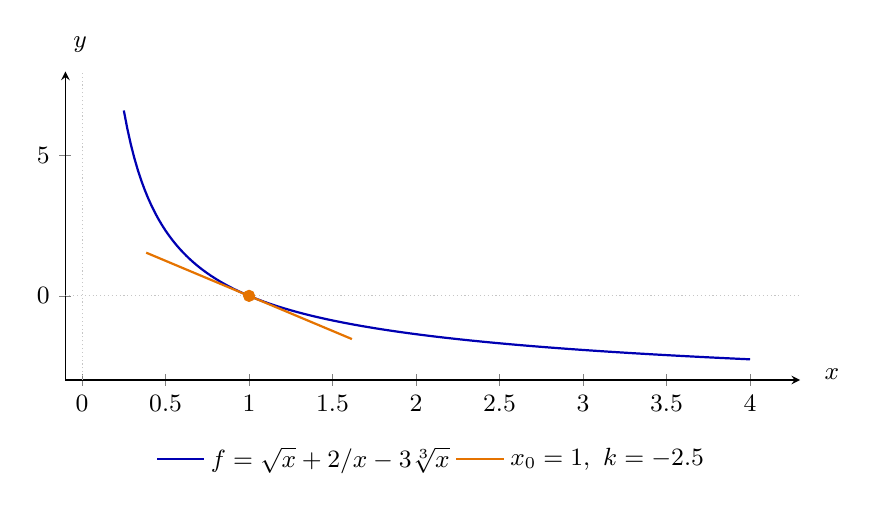
\begin{tikzpicture}[font=\small,>=stealth]
\begin{axis}[width=.90\linewidth,height=5.5cm,xmin=-0.1,xmax=4.3,ymin=-3,ymax=8,
axis lines=left,xlabel={$x$},ylabel={$y$},font=\small,
xlabel style={at={(axis description cs:1.02,.02)},anchor=west},
ylabel style={rotate=-90,at={(axis description cs:.02,1.03)},anchor=south},
legend style={at={(axis description cs:.5,-.18)},anchor=north,draw=none,fill=none,font=\small,legend columns=2},
unbounded coords=jump,clip=true,]
\addplot[gray!45,thin,densely dotted,forget plot] coordinates {(-0.1,0) (4.3,0)};
\addplot[gray!45,thin,densely dotted,forget plot] coordinates {(0,-3) (0,8)};
\addplot[blue!70!black,thick] coordinates {(0.25,6.6101184) (0.27083333,5.9640479) (0.29166667,5.407676) (0.3125,4.9232038) (0.33333333,4.4972664) (0.35416667,4.1196317) (0.375,3.7823314) (0.39583333,3.4790674) (0.41666667,3.2047949) (0.4375,2.9554247) (0.45833333,2.7276071) (0.47916667,2.5185712) (0.5,2.3260052) (0.52083333,2.1479644) (0.54166667,1.9828011) (0.5625,1.8291101) (0.58333333,1.6856851) (0.60416667,1.5514848) (0.625,1.4256055) (0.64583333,1.3072592) (0.66666667,1.1957552) (0.6875,1.0904859) (0.70833333,0.9909142) (0.72916667,0.89656396) (0.75,0.80701118) (0.77083333,0.72187721) (0.79166667,0.64082276) (0.8125,0.56354291) (0.83333333,0.48976284) (0.85416667,0.41923417) (0.875,0.35173186) (0.89583333,0.28705148) (0.91666667,0.22500695) (0.9375,0.16542844) (0.95833333,0.10816068) (0.97916667,0.053061406) (1,0) (1.0208333,-0.051143664) (1.0416667,-0.10048027) (1.0625,-0.14811198) (1.0833333,-0.19413323) (1.1041667,-0.23863147) (1.125,-0.28168779) (1.1458333,-0.3233775) (1.1666667,-0.36377063) (1.1875,-0.40293243) (1.2083333,-0.44092369) (1.2291667,-0.4778012) (1.25,-0.51361805) (1.2708333,-0.5484239) (1.2916667,-0.5822653) (1.3125,-0.61518591) (1.3333333,-0.64722671) (1.3541667,-0.67842624) (1.375,-0.70882074) (1.3958333,-0.73844436) (1.4166667,-0.76732927) (1.4375,-0.79550585) (1.4583333,-0.82300276) (1.4791667,-0.8498471) (1.5,-0.87606452) (1.5208333,-0.90167928) (1.5416667,-0.92671438) (1.5625,-0.95119163) (1.5833333,-0.97513169) (1.6041667,-0.99855424) (1.625,-1.0214779) (1.6458333,-1.0439205) (1.6666667,-1.0658989) (1.6875,-1.0874291) (1.7083333,-1.1085265) (1.7291667,-1.1292057) (1.75,-1.1494806) (1.7708333,-1.1693645) (1.7916667,-1.1888702) (1.8125,-1.2080097) (1.8333333,-1.2267947) (1.8541667,-1.2452363) (1.875,-1.2633451) (1.8958333,-1.2811312) (1.9166667,-1.2986044) (1.9375,-1.3157741) (1.9583333,-1.3326491) (1.9791667,-1.3492382) (2,-1.3655496) (2.0208333,-1.3815911) (2.0416667,-1.3973705) (2.0625,-1.4128949) (2.0833333,-1.4281715) (2.1041667,-1.443207) (2.125,-1.4580079) (2.1458333,-1.4725806) (2.1666667,-1.486931) (2.1875,-1.5010649) (2.2083333,-1.514988) (2.2291667,-1.5287057) (2.25,-1.5422232) (2.2708333,-1.5555455) (2.2916667,-1.5686775) (2.3125,-1.5816239) (2.3333333,-1.5943891) (2.3541667,-1.6069777) (2.375,-1.6193937) (2.3958333,-1.6316414) (2.4166667,-1.6437246) (2.4375,-1.6556471) (2.4583333,-1.6674128) (2.4791667,-1.6790251) (2.5,-1.6904876) (2.5208333,-1.7018036) (2.5416667,-1.7129763) (2.5625,-1.7240089) (2.5833333,-1.7349045) (2.6041667,-1.745666) (2.625,-1.7562963) (2.6458333,-1.7667983) (2.6666667,-1.7771745) (2.6875,-1.7874276) (2.7083333,-1.7975603) (2.7291667,-1.8075749) (2.75,-1.8174739) (2.7708333,-1.8272596) (2.7916667,-1.8369342) (2.8125,-1.8465) (2.8333333,-1.8559592) (2.8541667,-1.8653138) (2.875,-1.8745658) (2.8958333,-1.8837172) (2.9166667,-1.89277) (2.9375,-1.901726) (2.9583333,-1.910587) (2.9791667,-1.9193549) (3,-1.9280312) (3.0208333,-1.9366178) (3.0416667,-1.9451162) (3.0625,-1.9535281) (3.0833333,-1.9618549) (3.1041667,-1.9700983) (3.125,-1.9782597) (3.1458333,-1.9863404) (3.1666667,-1.9943421) (3.1875,-2.0022659) (3.2083333,-2.0101133) (3.2291667,-2.0178855) (3.25,-2.0255838) (3.2708333,-2.0332096) (3.2916667,-2.0407639) (3.3125,-2.0482479) (3.3333333,-2.0556629) (3.3541667,-2.0630099) (3.375,-2.0702901) (3.3958333,-2.0775045) (3.4166667,-2.0846542) (3.4375,-2.0917402) (3.4583333,-2.0987636) (3.4791667,-2.1057253) (3.5,-2.1126262) (3.5208333,-2.1194673) (3.5416667,-2.1262496) (3.5625,-2.1329739) (3.5833333,-2.1396412) (3.6041667,-2.1462522) (3.625,-2.1528078) (3.6458333,-2.1593089) (3.6666667,-2.1657562) (3.6875,-2.1721506) (3.7083333,-2.1784928) (3.7291667,-2.1847836) (3.75,-2.1910238) (3.7708333,-2.1972139) (3.7916667,-2.2033549) (3.8125,-2.2094472) (3.8333333,-2.2154918) (3.8541667,-2.2214891) (3.875,-2.22744) (3.8958333,-2.2333449) (3.9166667,-2.2392046) (3.9375,-2.2450197) (3.9583333,-2.2507908) (3.9791667,-2.2565184) (4,-2.2622032)};
\addlegendentry{$f=\sqrt x+2/x-3\sqrt[3]x$}
\addplot[orange!90!black,thick] coordinates {(0.384,1.54) (1.616,-1.54)};
\addlegendentry{$x_0=1,\ k=-2.5$}
\addplot[only marks,mark=*,orange!90!black,forget plot] coordinates {(1,0)};

\end{axis}
\end{tikzpicture}
\par\smallskip{\small 按本题原函数绘图；切线斜率由本题的导函数计算。}
\end{center}


\end{minipage}

第一步：根式要求 $x\ge0$，分母要求 $x\ne0$，故 $x>0$。

第二步：逐项应用公式，
\[
\begin{aligned}
f'(x)&=(\sqrt x)'+2(1/x)'-3(\sqrt[3]x)'\\
&=\frac1{2\sqrt x}-\frac2{x^2}-\frac1{\sqrt[3]{x^2}}.
\end{aligned}
\]
\textbf{关键结论：} 先确定原函数定义域，再改写为幂函数。

\medskip
\end{examplebox}

\begin{examplebox}
\begin{minipage}{\linewidth}
\textbf{\textcolor{CExample}{例 5（正切与余切）}}

求 $f(x)=\tan x+\cot x$ 的导数并求 $f'(\pi/4)$。
% F049: native TikZ/PGFPlots, computed from the stated mathematical model.
\begin{center}
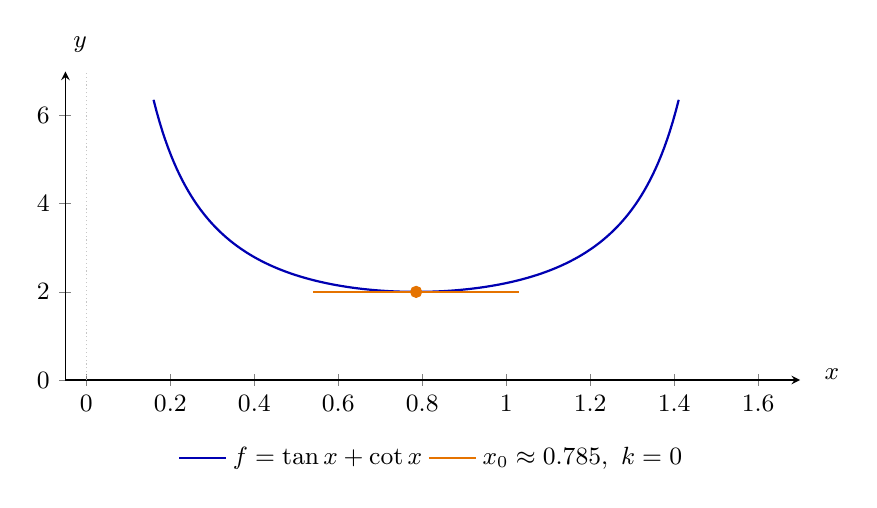
\begin{tikzpicture}[font=\small,>=stealth]
\begin{axis}[width=.90\linewidth,height=5.5cm,xmin=-0.05,xmax=1.7,ymin=0,ymax=7,
axis lines=left,xlabel={$x$},ylabel={$y$},font=\small,
xlabel style={at={(axis description cs:1.02,.02)},anchor=west},
ylabel style={rotate=-90,at={(axis description cs:.02,1.03)},anchor=south},
legend style={at={(axis description cs:.5,-.18)},anchor=north,draw=none,fill=none,font=\small,legend columns=2},
unbounded coords=jump,clip=true,]
\addplot[gray!45,thin,densely dotted,forget plot] coordinates {(0,0) (0,7)};
\addplot[blue!70!black,thick] coordinates {(0.16,6.3579549) (0.16694887,6.102622) (0.17389774,5.8680951) (0.18084661,5.6519783) (0.18779547,5.4522305) (0.19474434,5.267102) (0.20169321,5.0950844) (0.20864208,4.9348702) (0.21559095,4.7853208) (0.22253982,4.6454396) (0.22948868,4.5143512) (0.23643755,4.3912829) (0.24338642,4.2755505) (0.25033529,4.1665458) (0.25728416,4.0637264) (0.26423303,3.9666071) (0.2711819,3.8747525) (0.27813076,3.7877708) (0.28507963,3.7053085) (0.2920285,3.6270458) (0.29897737,3.5526928) (0.30592624,3.481986) (0.31287511,3.4146853) (0.31982398,3.3505719) (0.32677284,3.2894452) (0.33372171,3.2311219) (0.34067058,3.1754333) (0.34761945,3.1222246) (0.35456832,3.0713531) (0.36151719,3.0226873) (0.36846605,2.9761054) (0.37541492,2.9314951) (0.38236379,2.8887522) (0.38931266,2.8477799) (0.39626153,2.8084884) (0.4032104,2.7707943) (0.41015927,2.7346198) (0.41710813,2.6998924) (0.424057,2.6665446) (0.43100587,2.6345131) (0.43795474,2.603739) (0.44490361,2.5741669) (0.45185248,2.5457452) (0.45880134,2.5184254) (0.46575021,2.492162) (0.47269908,2.4669123) (0.47964795,2.4426361) (0.48659682,2.4192957) (0.49354569,2.3968558) (0.50049456,2.3752828) (0.50744342,2.3545455) (0.51439229,2.3346141) (0.52134116,2.3154608) (0.52829003,2.2970592) (0.5352389,2.2793846) (0.54218777,2.2624136) (0.54913664,2.246124) (0.5560855,2.230495) (0.56303437,2.215507) (0.56998324,2.2011414) (0.57693211,2.1873806) (0.58388098,2.1742082) (0.59082985,2.1616084) (0.59777871,2.1495666) (0.60472758,2.138069) (0.61167645,2.1271023) (0.61862532,2.1166542) (0.62557419,2.1067132) (0.63252306,2.0972684) (0.63947193,2.0883094) (0.64642079,2.0798266) (0.65336966,2.0718109) (0.66031853,2.064254) (0.6672674,2.0571479) (0.67421627,2.0504853) (0.68116514,2.0442592) (0.688114,2.0384633) (0.69506287,2.0330918) (0.70201174,2.0281392) (0.70896061,2.0236006) (0.71590948,2.0194714) (0.72285835,2.0157476) (0.72980722,2.0124254) (0.73675608,2.0095017) (0.74370495,2.0069735) (0.75065382,2.0048384) (0.75760269,2.0030943) (0.76455156,2.0017396) (0.77150043,2.0007728) (0.77844929,2.0001932) (0.78539816,2) (0.79234703,2.0001932) (0.7992959,2.0007728) (0.80624477,2.0017396) (0.81319364,2.0030943) (0.82014251,2.0048384) (0.82709137,2.0069735) (0.83404024,2.0095017) (0.84098911,2.0124254) (0.84793798,2.0157476) (0.85488685,2.0194714) (0.86183572,2.0236006) (0.86878459,2.0281392) (0.87573345,2.0330918) (0.88268232,2.0384633) (0.88963119,2.0442592) (0.89658006,2.0504853) (0.90352893,2.0571479) (0.9104778,2.064254) (0.91742666,2.0718109) (0.92437553,2.0798266) (0.9313244,2.0883094) (0.93827327,2.0972684) (0.94522214,2.1067132) (0.95217101,2.1166542) (0.95911988,2.1271023) (0.96606874,2.138069) (0.97301761,2.1495666) (0.97996648,2.1616084) (0.98691535,2.1742082) (0.99386422,2.1873806) (1.0008131,2.2011414) (1.007762,2.215507) (1.0147108,2.230495) (1.0216597,2.246124) (1.0286086,2.2624136) (1.0355574,2.2793846) (1.0425063,2.2970592) (1.0494552,2.3154608) (1.056404,2.3346141) (1.0633529,2.3545455) (1.0703018,2.3752828) (1.0772506,2.3968558) (1.0841995,2.4192957) (1.0911484,2.4426361) (1.0980972,2.4669123) (1.1050461,2.492162) (1.111995,2.5184254) (1.1189439,2.5457452) (1.1258927,2.5741669) (1.1328416,2.603739) (1.1397905,2.6345131) (1.1467393,2.6665446) (1.1536882,2.6998924) (1.1606371,2.7346198) (1.1675859,2.7707943) (1.1745348,2.8084884) (1.1814837,2.8477799) (1.1884325,2.8887522) (1.1953814,2.9314951) (1.2023303,2.9761054) (1.2092791,3.0226873) (1.216228,3.0713531) (1.2231769,3.1222246) (1.2301257,3.1754333) (1.2370746,3.2311219) (1.2440235,3.2894452) (1.2509724,3.3505719) (1.2579212,3.4146853) (1.2648701,3.481986) (1.271819,3.5526928) (1.2787678,3.6270458) (1.2857167,3.7053085) (1.2926656,3.7877708) (1.2996144,3.8747525) (1.3065633,3.9666071) (1.3135122,4.0637264) (1.320461,4.1665458) (1.3274099,4.2755505) (1.3343588,4.3912829) (1.3413076,4.5143512) (1.3482565,4.6454396) (1.3552054,4.7853208) (1.3621542,4.9348702) (1.3691031,5.0950844) (1.376052,5.267102) (1.3830009,5.4522305) (1.3899497,5.6519783) (1.3968986,5.8680951) (1.4038475,6.102622) (1.4107963,6.3579549)};
\addlegendentry{$f=\tan x+\cot x$}
\addplot[orange!90!black,thick] coordinates {(0.54039816,2) (1.0303982,2)};
\addlegendentry{$x_0\approx0.785,\ k=0$}
\addplot[only marks,mark=*,orange!90!black,forget plot] coordinates {(0.78539816,2)};

\end{axis}
\end{tikzpicture}
\par\smallskip{\small 按本题原函数绘图；切线斜率由本题的导函数计算。}
\end{center}


\end{minipage}

第一步：$\sin x\cos x\ne0$。第二步：
\[
f'(x)=\frac1{\cos^2x}-\frac1{\sin^2x}.
\]
第三步：$\sin(\pi/4)=\cos(\pi/4)=\sqrt2/2$，故 $f'(\pi/4)=2-2=0$。

\textbf{关键结论：} 正切、余切导数符号相反。

\medskip
\end{examplebox}

\begin{examplebox}
\begin{minipage}{\linewidth}
\textbf{\textcolor{CExample}{例 6（绝对值的折点）}}

判断 $f(x)=|x-2|$ 在 $x=2$ 处是否可导，并写出其他点的导数。
% F049: native TikZ/PGFPlots, computed from the stated mathematical model.
\begin{center}
\begin{tikzpicture}[font=\small,>=stealth]
\begin{axis}[width=.90\linewidth,height=5.5cm,xmin=-0.3,xmax=4.3,ymin=-0.4,ymax=2.7,
axis lines=left,xlabel={$x$},ylabel={$y$},font=\small,
xlabel style={at={(axis description cs:1.02,.02)},anchor=west},
ylabel style={rotate=-90,at={(axis description cs:.02,1.03)},anchor=south},
legend style={at={(axis description cs:.5,-.18)},anchor=north,draw=none,fill=none,font=\small,legend columns=2},
unbounded coords=jump,clip=true,]
\addplot[gray!45,thin,densely dotted,forget plot] coordinates {(-0.3,0) (4.3,0)};
\addplot[gray!45,thin,densely dotted,forget plot] coordinates {(0,-0.4) (0,2.7)};
\addplot[blue!70!black,thick] coordinates {(0,2) (0.011111111,1.9888889) (0.022222222,1.9777778) (0.033333333,1.9666667) (0.044444444,1.9555556) (0.055555556,1.9444444) (0.066666667,1.9333333) (0.077777778,1.9222222) (0.088888889,1.9111111) (0.1,1.9) (0.11111111,1.8888889) (0.12222222,1.8777778) (0.13333333,1.8666667) (0.14444444,1.8555556) (0.15555556,1.8444444) (0.16666667,1.8333333) (0.17777778,1.8222222) (0.18888889,1.8111111) (0.2,1.8) (0.21111111,1.7888889) (0.22222222,1.7777778) (0.23333333,1.7666667) (0.24444444,1.7555556) (0.25555556,1.7444444) (0.26666667,1.7333333) (0.27777778,1.7222222) (0.28888889,1.7111111) (0.3,1.7) (0.31111111,1.6888889) (0.32222222,1.6777778) (0.33333333,1.6666667) (0.34444444,1.6555556) (0.35555556,1.6444444) (0.36666667,1.6333333) (0.37777778,1.6222222) (0.38888889,1.6111111) (0.4,1.6) (0.41111111,1.5888889) (0.42222222,1.5777778) (0.43333333,1.5666667) (0.44444444,1.5555556) (0.45555556,1.5444444) (0.46666667,1.5333333) (0.47777778,1.5222222) (0.48888889,1.5111111) (0.5,1.5) (0.51111111,1.4888889) (0.52222222,1.4777778) (0.53333333,1.4666667) (0.54444444,1.4555556) (0.55555556,1.4444444) (0.56666667,1.4333333) (0.57777778,1.4222222) (0.58888889,1.4111111) (0.6,1.4) (0.61111111,1.3888889) (0.62222222,1.3777778) (0.63333333,1.3666667) (0.64444444,1.3555556) (0.65555556,1.3444444) (0.66666667,1.3333333) (0.67777778,1.3222222) (0.68888889,1.3111111) (0.7,1.3) (0.71111111,1.2888889) (0.72222222,1.2777778) (0.73333333,1.2666667) (0.74444444,1.2555556) (0.75555556,1.2444444) (0.76666667,1.2333333) (0.77777778,1.2222222) (0.78888889,1.2111111) (0.8,1.2) (0.81111111,1.1888889) (0.82222222,1.1777778) (0.83333333,1.1666667) (0.84444444,1.1555556) (0.85555556,1.1444444) (0.86666667,1.1333333) (0.87777778,1.1222222) (0.88888889,1.1111111) (0.9,1.1) (0.91111111,1.0888889) (0.92222222,1.0777778) (0.93333333,1.0666667) (0.94444444,1.0555556) (0.95555556,1.0444444) (0.96666667,1.0333333) (0.97777778,1.0222222) (0.98888889,1.0111111) (1,1) (1.0111111,0.98888889) (1.0222222,0.97777778) (1.0333333,0.96666667) (1.0444444,0.95555556) (1.0555556,0.94444444) (1.0666667,0.93333333) (1.0777778,0.92222222) (1.0888889,0.91111111) (1.1,0.9) (1.1111111,0.88888889) (1.1222222,0.87777778) (1.1333333,0.86666667) (1.1444444,0.85555556) (1.1555556,0.84444444) (1.1666667,0.83333333) (1.1777778,0.82222222) (1.1888889,0.81111111) (1.2,0.8) (1.2111111,0.78888889) (1.2222222,0.77777778) (1.2333333,0.76666667) (1.2444444,0.75555556) (1.2555556,0.74444444) (1.2666667,0.73333333) (1.2777778,0.72222222) (1.2888889,0.71111111) (1.3,0.7) (1.3111111,0.68888889) (1.3222222,0.67777778) (1.3333333,0.66666667) (1.3444444,0.65555556) (1.3555556,0.64444444) (1.3666667,0.63333333) (1.3777778,0.62222222) (1.3888889,0.61111111) (1.4,0.6) (1.4111111,0.58888889) (1.4222222,0.57777778) (1.4333333,0.56666667) (1.4444444,0.55555556) (1.4555556,0.54444444) (1.4666667,0.53333333) (1.4777778,0.52222222) (1.4888889,0.51111111) (1.5,0.5) (1.5111111,0.48888889) (1.5222222,0.47777778) (1.5333333,0.46666667) (1.5444444,0.45555556) (1.5555556,0.44444444) (1.5666667,0.43333333) (1.5777778,0.42222222) (1.5888889,0.41111111) (1.6,0.4) (1.6111111,0.38888889) (1.6222222,0.37777778) (1.6333333,0.36666667) (1.6444444,0.35555556) (1.6555556,0.34444444) (1.6666667,0.33333333) (1.6777778,0.32222222) (1.6888889,0.31111111) (1.7,0.3) (1.7111111,0.28888889) (1.7222222,0.27777778) (1.7333333,0.26666667) (1.7444444,0.25555556) (1.7555556,0.24444444) (1.7666667,0.23333333) (1.7777778,0.22222222) (1.7888889,0.21111111) (1.8,0.2) (1.8111111,0.18888889) (1.8222222,0.17777778) (1.8333333,0.16666667) (1.8444444,0.15555556) (1.8555556,0.14444444) (1.8666667,0.13333333) (1.8777778,0.12222222) (1.8888889,0.11111111) (1.9,0.1) (1.9111111,0.088888889) (1.9222222,0.077777778) (1.9333333,0.066666667) (1.9444444,0.055555556) (1.9555556,0.044444444) (1.9666667,0.033333333) (1.9777778,0.022222222) (1.9888889,0.011111111) (2,0)};
\addlegendentry{$f=|x-2|$}
\addplot[blue!70!black,thick,forget plot] coordinates {(2,0) (2.0111111,0.011111111) (2.0222222,0.022222222) (2.0333333,0.033333333) (2.0444444,0.044444444) (2.0555556,0.055555556) (2.0666667,0.066666667) (2.0777778,0.077777778) (2.0888889,0.088888889) (2.1,0.1) (2.1111111,0.11111111) (2.1222222,0.12222222) (2.1333333,0.13333333) (2.1444444,0.14444444) (2.1555556,0.15555556) (2.1666667,0.16666667) (2.1777778,0.17777778) (2.1888889,0.18888889) (2.2,0.2) (2.2111111,0.21111111) (2.2222222,0.22222222) (2.2333333,0.23333333) (2.2444444,0.24444444) (2.2555556,0.25555556) (2.2666667,0.26666667) (2.2777778,0.27777778) (2.2888889,0.28888889) (2.3,0.3) (2.3111111,0.31111111) (2.3222222,0.32222222) (2.3333333,0.33333333) (2.3444444,0.34444444) (2.3555556,0.35555556) (2.3666667,0.36666667) (2.3777778,0.37777778) (2.3888889,0.38888889) (2.4,0.4) (2.4111111,0.41111111) (2.4222222,0.42222222) (2.4333333,0.43333333) (2.4444444,0.44444444) (2.4555556,0.45555556) (2.4666667,0.46666667) (2.4777778,0.47777778) (2.4888889,0.48888889) (2.5,0.5) (2.5111111,0.51111111) (2.5222222,0.52222222) (2.5333333,0.53333333) (2.5444444,0.54444444) (2.5555556,0.55555556) (2.5666667,0.56666667) (2.5777778,0.57777778) (2.5888889,0.58888889) (2.6,0.6) (2.6111111,0.61111111) (2.6222222,0.62222222) (2.6333333,0.63333333) (2.6444444,0.64444444) (2.6555556,0.65555556) (2.6666667,0.66666667) (2.6777778,0.67777778) (2.6888889,0.68888889) (2.7,0.7) (2.7111111,0.71111111) (2.7222222,0.72222222) (2.7333333,0.73333333) (2.7444444,0.74444444) (2.7555556,0.75555556) (2.7666667,0.76666667) (2.7777778,0.77777778) (2.7888889,0.78888889) (2.8,0.8) (2.8111111,0.81111111) (2.8222222,0.82222222) (2.8333333,0.83333333) (2.8444444,0.84444444) (2.8555556,0.85555556) (2.8666667,0.86666667) (2.8777778,0.87777778) (2.8888889,0.88888889) (2.9,0.9) (2.9111111,0.91111111) (2.9222222,0.92222222) (2.9333333,0.93333333) (2.9444444,0.94444444) (2.9555556,0.95555556) (2.9666667,0.96666667) (2.9777778,0.97777778) (2.9888889,0.98888889) (3,1) (3.0111111,1.0111111) (3.0222222,1.0222222) (3.0333333,1.0333333) (3.0444444,1.0444444) (3.0555556,1.0555556) (3.0666667,1.0666667) (3.0777778,1.0777778) (3.0888889,1.0888889) (3.1,1.1) (3.1111111,1.1111111) (3.1222222,1.1222222) (3.1333333,1.1333333) (3.1444444,1.1444444) (3.1555556,1.1555556) (3.1666667,1.1666667) (3.1777778,1.1777778) (3.1888889,1.1888889) (3.2,1.2) (3.2111111,1.2111111) (3.2222222,1.2222222) (3.2333333,1.2333333) (3.2444444,1.2444444) (3.2555556,1.2555556) (3.2666667,1.2666667) (3.2777778,1.2777778) (3.2888889,1.2888889) (3.3,1.3) (3.3111111,1.3111111) (3.3222222,1.3222222) (3.3333333,1.3333333) (3.3444444,1.3444444) (3.3555556,1.3555556) (3.3666667,1.3666667) (3.3777778,1.3777778) (3.3888889,1.3888889) (3.4,1.4) (3.4111111,1.4111111) (3.4222222,1.4222222) (3.4333333,1.4333333) (3.4444444,1.4444444) (3.4555556,1.4555556) (3.4666667,1.4666667) (3.4777778,1.4777778) (3.4888889,1.4888889) (3.5,1.5) (3.5111111,1.5111111) (3.5222222,1.5222222) (3.5333333,1.5333333) (3.5444444,1.5444444) (3.5555556,1.5555556) (3.5666667,1.5666667) (3.5777778,1.5777778) (3.5888889,1.5888889) (3.6,1.6) (3.6111111,1.6111111) (3.6222222,1.6222222) (3.6333333,1.6333333) (3.6444444,1.6444444) (3.6555556,1.6555556) (3.6666667,1.6666667) (3.6777778,1.6777778) (3.6888889,1.6888889) (3.7,1.7) (3.7111111,1.7111111) (3.7222222,1.7222222) (3.7333333,1.7333333) (3.7444444,1.7444444) (3.7555556,1.7555556) (3.7666667,1.7666667) (3.7777778,1.7777778) (3.7888889,1.7888889) (3.8,1.8) (3.8111111,1.8111111) (3.8222222,1.8222222) (3.8333333,1.8333333) (3.8444444,1.8444444) (3.8555556,1.8555556) (3.8666667,1.8666667) (3.8777778,1.8777778) (3.8888889,1.8888889) (3.9,1.9) (3.9111111,1.9111111) (3.9222222,1.9222222) (3.9333333,1.9333333) (3.9444444,1.9444444) (3.9555556,1.9555556) (3.9666667,1.9666667) (3.9777778,1.9777778) (3.9888889,1.9888889) (4,2)};
\addplot[orange!90!black,thick] coordinates {(0.356,1.644) (1.644,0.356)};
\addlegendentry{$x_0=1,\ k=-1$}
\addplot[only marks,mark=*,orange!90!black,forget plot] coordinates {(1,1)};
\addplot[purple,thick,dashed] coordinates {(2.356,0.356) (3.644,1.644)};
\addlegendentry{$x_0=3,\ k=1$}
\addplot[only marks,mark=*,purple,forget plot] coordinates {(3,1)};

\end{axis}
\end{tikzpicture}
\par\smallskip{\small 按本题原函数绘图；切线斜率由本题的导函数计算。}
\end{center}


\end{minipage}
\[
f(x)=\begin{cases}2-x,&x<2,\\x-2,&x\ge2.\end{cases}
\]
当 $x<2$，$f'(x)=-1$；当 $x>2$，$f'(x)=1$。在 $x=2$ 处，差商是 $|h|/h$，左极限为 $-1$，右极限为 $1$，故不可导。

\textbf{关键结论：} 连续不等于可导，折点要比较左右差商。

\medskip
\end{examplebox}

\begin{examplebox}
\begin{minipage}{\linewidth}
\textbf{\textcolor{CExample}{例 7（变指数与单调性）}}

求 $y=x^x$（$x>0$）的最小值。
% F049: native TikZ/PGFPlots, computed from the stated mathematical model.
\begin{center}
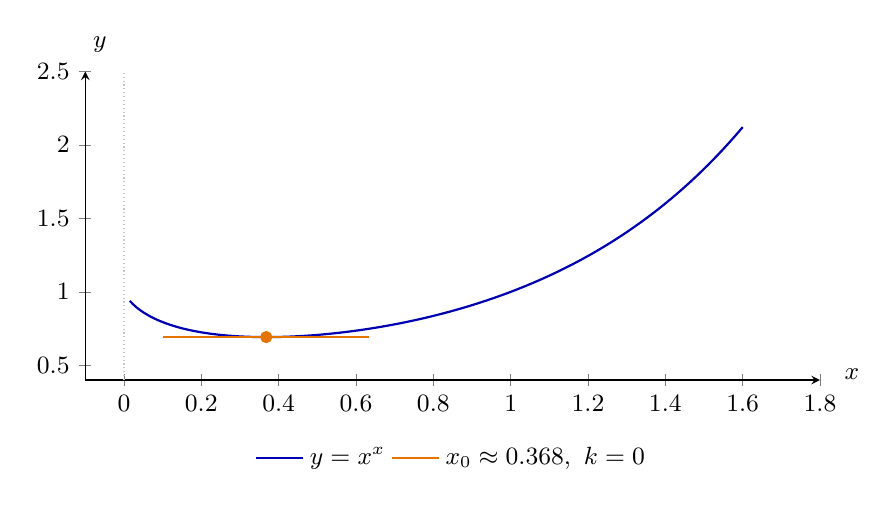
\begin{tikzpicture}[font=\small,>=stealth]
\begin{axis}[width=.90\linewidth,height=5.5cm,xmin=-0.1,xmax=1.8,ymin=0.4,ymax=2.5,
axis lines=left,xlabel={$x$},ylabel={$y$},font=\small,
xlabel style={at={(axis description cs:1.02,.02)},anchor=west},
ylabel style={rotate=-90,at={(axis description cs:.02,1.03)},anchor=south},
legend style={at={(axis description cs:.5,-.18)},anchor=north,draw=none,fill=none,font=\small,legend columns=2},
unbounded coords=jump,clip=true,]
\addplot[gray!45,thin,densely dotted,forget plot] coordinates {(0,0.4) (0,2.5)};
\addplot[blue!70!black,thick] coordinates {(0.015,0.93894763) (0.023805556,0.91486271) (0.032611111,0.89437407) (0.041416667,0.87645173) (0.050222222,0.86051037) (0.059027778,0.84617111) (0.067833333,0.8331686) (0.076638889,0.82130681) (0.085444444,0.81043524) (0.09425,0.8004349) (0.10305556,0.79120956) (0.11186111,0.78267992) (0.12066667,0.77477965) (0.12947222,0.76745255) (0.13827778,0.76065049) (0.14708333,0.75433187) (0.15588889,0.74846044) (0.16469444,0.74300438) (0.1735,0.7379356) (0.18230556,0.73322914) (0.19111111,0.72886275) (0.19991667,0.72481649) (0.20872222,0.72107239) (0.21752778,0.71761424) (0.22633333,0.71442737) (0.23513889,0.71149841) (0.24394444,0.70881521) (0.25275,0.70636666) (0.26155556,0.70414259) (0.27036111,0.70213368) (0.27916667,0.70033137) (0.28797222,0.69872775) (0.29677778,0.69731556) (0.30558333,0.6960881) (0.31438889,0.69503915) (0.32319444,0.69416299) (0.332,0.6934543) (0.34080556,0.69290816) (0.34961111,0.69252001) (0.35841667,0.69228561) (0.36722222,0.69220103) (0.37602778,0.69226264) (0.38483333,0.69246704) (0.39363889,0.69281108) (0.40244444,0.69329186) (0.41125,0.69390666) (0.42005556,0.69465298) (0.42886111,0.69552848) (0.43766667,0.69653101) (0.44647222,0.69765859) (0.45527778,0.69890937) (0.46408333,0.70028165) (0.47288889,0.70177388) (0.48169444,0.70338461) (0.4905,0.70511253) (0.49930556,0.70695646) (0.50811111,0.70891529) (0.51691667,0.71098804) (0.52572222,0.71317383) (0.53452778,0.71547186) (0.54333333,0.71788143) (0.55213889,0.72040191) (0.56094444,0.72303278) (0.56975,0.72577357) (0.57855556,0.72862391) (0.58736111,0.73158349) (0.59616667,0.73465207) (0.60497222,0.73782948) (0.61377778,0.74111561) (0.62258333,0.74451043) (0.63138889,0.74801396) (0.64019444,0.75162628) (0.649,0.75534752) (0.65780556,0.75917789) (0.66661111,0.76311762) (0.67541667,0.76716704) (0.68422222,0.77132649) (0.69302778,0.77559638) (0.70183333,0.77997717) (0.71063889,0.78446937) (0.71944444,0.78907353) (0.72825,0.79379027) (0.73705556,0.79862022) (0.74586111,0.8035641) (0.75466667,0.80862265) (0.76347222,0.81379664) (0.77227778,0.81908693) (0.78108333,0.82449439) (0.78988889,0.83001994) (0.79869444,0.83566455) (0.8075,0.84142923) (0.81630556,0.84731503) (0.82511111,0.85332306) (0.83391667,0.85945445) (0.84272222,0.86571039) (0.85152778,0.87209211) (0.86033333,0.87860087) (0.86913889,0.88523798) (0.87794444,0.89200481) (0.88675,0.89890276) (0.89555556,0.90593325) (0.90436111,0.91309779) (0.91316667,0.9203979) (0.92197222,0.92783516) (0.93077778,0.93541118) (0.93958333,0.94312762) (0.94838889,0.95098619) (0.95719444,0.95898865) (0.966,0.96713679) (0.97480556,0.97543245) (0.98361111,0.98387753) (0.99241667,0.99247396) (1.0012222,1.0012237) (1.0100278,1.0101288) (1.0188333,1.0191914) (1.0276389,1.0284135) (1.0364444,1.0377974) (1.04525,1.0473453) (1.0540556,1.0570594) (1.0628611,1.0669421) (1.0716667,1.0769958) (1.0804722,1.0872228) (1.0892778,1.0976258) (1.0980833,1.1082071) (1.1068889,1.1189695) (1.1156944,1.1299156) (1.1245,1.141048) (1.1333056,1.1523696) (1.1421111,1.1638831) (1.1509167,1.1755914) (1.1597222,1.1874976) (1.1685278,1.1996045) (1.1773333,1.2119153) (1.1861389,1.2244331) (1.1949444,1.237161) (1.20375,1.2501023) (1.2125556,1.2632604) (1.2213611,1.2766387) (1.2301667,1.2902405) (1.2389722,1.3040694) (1.2477778,1.318129) (1.2565833,1.332423) (1.2653889,1.3469551) (1.2741944,1.3617292) (1.283,1.3767491) (1.2918056,1.3920188) (1.3006111,1.4075423) (1.3094167,1.4233238) (1.3182222,1.4393674) (1.3270278,1.4556776) (1.3358333,1.4722585) (1.3446389,1.4891148) (1.3534444,1.5062509) (1.36225,1.5236715) (1.3710556,1.5413813) (1.3798611,1.5593852) (1.3886667,1.5776879) (1.3974722,1.5962947) (1.4062778,1.6152105) (1.4150833,1.6344405) (1.4238889,1.6539901) (1.4326944,1.6738647) (1.4415,1.6940699) (1.4503056,1.7146111) (1.4591111,1.7354942) (1.4679167,1.7567249) (1.4767222,1.7783094) (1.4855278,1.8002535) (1.4943333,1.8225636) (1.5031389,1.8452459) (1.5119444,1.8683069) (1.52075,1.891753) (1.5295556,1.9155911) (1.5383611,1.9398279) (1.5471667,1.9644704) (1.5559722,1.9895256) (1.5647778,2.0150008) (1.5735833,2.0409033) (1.5823889,2.0672406) (1.5911944,2.0940205) (1.6,2.1212506)};
\addlegendentry{$y=x^x$}
\addplot[orange!90!black,thick] coordinates {(0.10187944,0.69220063) (0.63387944,0.69220063)};
\addlegendentry{$x_0\approx0.368,\ k=0$}
\addplot[only marks,mark=*,orange!90!black,forget plot] coordinates {(0.36787944,0.69220063)};

\end{axis}
\end{tikzpicture}
\par\smallskip{\small 按本题原函数绘图；切线斜率由本题的导函数计算。}
\end{center}


\end{minipage}
\[
\begin{aligned}
y&=e^{x\ln x},\\
y'&=e^{x\ln x}(\ln x+1)=x^x(\ln x+1).
\end{aligned}
\]
因 $x^x>0$，导数符号由 $\ln x+1$ 决定。令 $\ln x+1=0$ 得 $x=1/e$。在 $(0,1/e)$ 上导数为负，在 $(1/e,+\infty)$ 上导数为正，故最小值为 $(1/e)^{1/e}=e^{-1/e}$。

\medskip
\end{examplebox}

\begin{examplebox}
\begin{minipage}{\linewidth}
\textbf{\textcolor{CExample}{例 8（复合对数）}}

求 $f(x)=\ln|x^2-4|$ 的导数。
% F049: native TikZ/PGFPlots, computed from the stated mathematical model.
\begin{center}
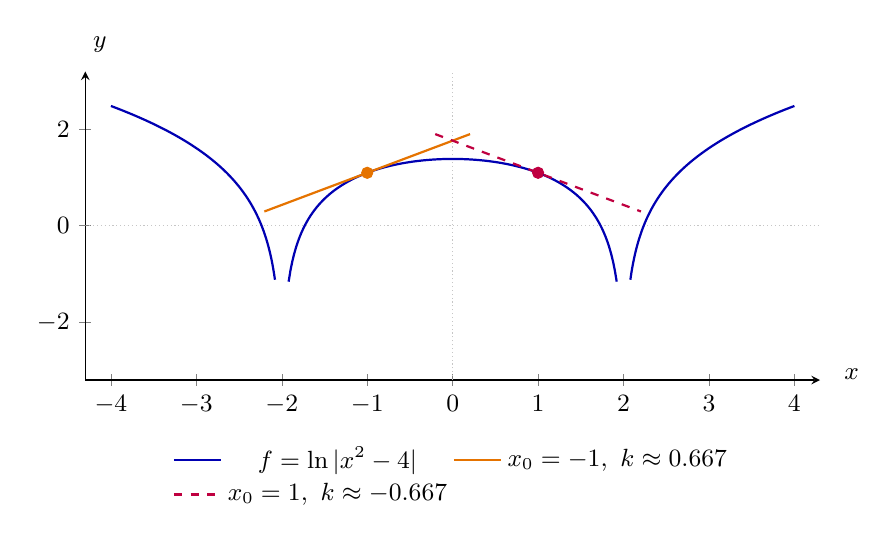
\begin{tikzpicture}[font=\small,>=stealth]
\begin{axis}[width=.90\linewidth,height=5.5cm,xmin=-4.3,xmax=4.3,ymin=-3.2,ymax=3.2,
axis lines=left,xlabel={$x$},ylabel={$y$},font=\small,
xlabel style={at={(axis description cs:1.02,.02)},anchor=west},
ylabel style={rotate=-90,at={(axis description cs:.02,1.03)},anchor=south},
legend style={at={(axis description cs:.5,-.18)},anchor=north,draw=none,fill=none,font=\small,legend columns=2},
unbounded coords=jump,clip=true,]
\addplot[gray!45,thin,densely dotted,forget plot] coordinates {(-4.3,0) (4.3,0)};
\addplot[gray!45,thin,densely dotted,forget plot] coordinates {(0,-3.2) (0,3.2)};
\addplot[blue!70!black,thick] coordinates {(-4,2.4849066) (-3.9893333,2.4777797) (-3.9786667,2.4706208) (-3.968,2.4634297) (-3.9573333,2.456206) (-3.9466667,2.4489493) (-3.936,2.4416595) (-3.9253333,2.4343361) (-3.9146667,2.4269787) (-3.904,2.419587) (-3.8933333,2.4121607) (-3.8826667,2.4046994) (-3.872,2.3972027) (-3.8613333,2.3896702) (-3.8506667,2.3821015) (-3.84,2.3744964) (-3.8293333,2.3668542) (-3.8186667,2.3591748) (-3.808,2.3514575) (-3.7973333,2.3437021) (-3.7866667,2.3359081) (-3.776,2.328075) (-3.7653333,2.3202025) (-3.7546667,2.31229) (-3.744,2.3043372) (-3.7333333,2.2963434) (-3.7226667,2.2883084) (-3.712,2.2802315) (-3.7013333,2.2721123) (-3.6906667,2.2639503) (-3.68,2.255745) (-3.6693333,2.2474959) (-3.6586667,2.2392024) (-3.648,2.2308639) (-3.6373333,2.22248) (-3.6266667,2.2140501) (-3.616,2.2055736) (-3.6053333,2.1970499) (-3.5946667,2.1884785) (-3.584,2.1798587) (-3.5733333,2.1711898) (-3.5626667,2.1624714) (-3.552,2.1537026) (-3.5413333,2.144883) (-3.5306667,2.1360117) (-3.52,2.1270882) (-3.5093333,2.1181117) (-3.4986667,2.1090815) (-3.488,2.0999968) (-3.4773333,2.090857) (-3.4666667,2.0816613) (-3.456,2.0724089) (-3.4453333,2.0630989) (-3.4346667,2.0537307) (-3.424,2.0443034) (-3.4133333,2.034816) (-3.4026667,2.0252678) (-3.392,2.0156579) (-3.3813333,2.0059854) (-3.3706667,1.9962493) (-3.36,1.9864487) (-3.3493333,1.9765826) (-3.3386667,1.96665) (-3.328,1.95665) (-3.3173333,1.9465814) (-3.3066667,1.9364433) (-3.296,1.9262344) (-3.2853333,1.9159538) (-3.2746667,1.9056002) (-3.264,1.8951725) (-3.2533333,1.8846695) (-3.2426667,1.8740899) (-3.232,1.8634325) (-3.2213333,1.852696) (-3.2106667,1.841879) (-3.2,1.8309802) (-3.1893333,1.8199982) (-3.1786667,1.8089315) (-3.168,1.7977787) (-3.1573333,1.7865382) (-3.1466667,1.7752084) (-3.136,1.7637879) (-3.1253333,1.7522749) (-3.1146667,1.7406676) (-3.104,1.7289645) (-3.0933333,1.7171636) (-3.0826667,1.7052632) (-3.072,1.6932613) (-3.0613333,1.6811559) (-3.0506667,1.6689451) (-3.04,1.6566268) (-3.0293333,1.6441988) (-3.0186667,1.6316589) (-3.008,1.6190048) (-2.9973333,1.6062342) (-2.9866667,1.5933447) (-2.976,1.5803337) (-2.9653333,1.5671986) (-2.9546667,1.5539369) (-2.944,1.5405456) (-2.9333333,1.527022) (-2.9226667,1.5133631) (-2.912,1.4995659) (-2.9013333,1.4856271) (-2.8906667,1.4715436) (-2.88,1.4573118) (-2.8693333,1.4429284) (-2.8586667,1.4283896) (-2.848,1.4136916) (-2.8373333,1.3988306) (-2.8266667,1.3838024) (-2.816,1.3686028) (-2.8053333,1.3532274) (-2.7946667,1.3376716) (-2.784,1.3219308) (-2.7733333,1.3059998) (-2.7626667,1.2898735) (-2.752,1.2735466) (-2.7413333,1.2570135) (-2.7306667,1.2402682) (-2.72,1.2233047) (-2.7093333,1.2061166) (-2.6986667,1.1886973) (-2.688,1.1710396) (-2.6773333,1.1531364) (-2.6666667,1.1349799) (-2.656,1.1165622) (-2.6453333,1.0978748) (-2.6346667,1.0789089) (-2.624,1.0596552) (-2.6133333,1.0401039) (-2.6026667,1.0202448) (-2.592,1.000067) (-2.5813333,0.97955911) (-2.5706667,0.95870906) (-2.56,0.93750413) (-2.5493333,0.91593084) (-2.5386667,0.89397495) (-2.528,0.87162135) (-2.5173333,0.84885398) (-2.5066667,0.82565583) (-2.496,0.80200876) (-2.4853333,0.77789348) (-2.4746667,0.75328939) (-2.464,0.7281745) (-2.4533333,0.70252529) (-2.4426667,0.67631656) (-2.432,0.64952126) (-2.4213333,0.62211032) (-2.4106667,0.59405243) (-2.4,0.56531381) (-2.3893333,0.53585795) (-2.3786667,0.5056453) (-2.368,0.4746329) (-2.3573333,0.44277402) (-2.3466667,0.41001769) (-2.336,0.37630815) (-2.3253333,0.34158423) (-2.3146667,0.30577867) (-2.304,0.26881725) (-2.2933333,0.23061777) (-2.2826667,0.19108894) (-2.272,0.15012889) (-2.2613333,0.10762355) (-2.2506667,0.06344459) (-2.24,0.017446914) (-2.2293333,-0.030534353) (-2.2186667,-0.080687656) (-2.208,-0.13322972) (-2.1973333,-0.18841153) (-2.1866667,-0.24652591) (-2.176,-0.30791743) (-2.1653333,-0.37299534) (-2.1546667,-0.44225081) (-2.144,-0.51628047) (-2.1333333,-0.59581884) (-2.1226667,-0.68178443) (-2.112,-0.77534688) (-2.1013333,-0.87802774) (-2.0906667,-0.99185755) (-2.08,-1.1196317)};
\addlegendentry{$f=\ln|x^2-4|$}
\addplot[blue!70!black,thick,forget plot] coordinates {(-1.92,-1.159637) (-1.8986667,-0.92870525) (-1.8773333,-0.743137) (-1.856,-0.5883116) (-1.8346667,-0.45570913) (-1.8133333,-0.33992709) (-1.792,-0.23732361) (-1.7706667,-0.14532691) (-1.7493333,-0.062053197) (-1.728,0.013918684) (-1.7066667,0.08368734) (-1.6853333,0.14811958) (-1.664,0.20791133) (-1.6426667,0.26362979) (-1.6213333,0.31574331) (-1.6,0.36464311) (-1.5786667,0.4106593) (-1.5573333,0.45407296) (-1.536,0.49512542) (-1.5146667,0.53402535) (-1.4933333,0.57095444) (-1.472,0.6060718) (-1.4506667,0.63951759) (-1.4293333,0.67141587) (-1.408,0.70187696) (-1.3866667,0.73099944) (-1.3653333,0.75887166) (-1.344,0.78557321) (-1.3226667,0.81117591) (-1.3013333,0.83574491) (-1.28,0.85933936) (-1.2586667,0.8820132) (-1.2373333,0.90381573) (-1.216,0.92479209) (-1.1946667,0.94498374) (-1.1733333,0.96442883) (-1.152,0.98316253) (-1.1306667,1.0012173) (-1.1093333,1.0186233) (-1.088,1.0354083) (-1.0666667,1.0515983) (-1.0453333,1.0672173) (-1.024,1.0822878) (-1.0026667,1.0968306) (-0.98133333,1.1108652) (-0.96,1.12441) (-0.93866667,1.1374819) (-0.91733333,1.1500971) (-0.896,1.1622704) (-0.87466667,1.174016) (-0.85333333,1.1853471) (-0.832,1.1962761) (-0.81066667,1.2068146) (-0.78933333,1.2169738) (-0.768,1.2267639) (-0.74666667,1.2361947) (-0.72533333,1.2452755) (-0.704,1.2540148) (-0.68266667,1.2624208) (-0.66133333,1.2705013) (-0.64,1.2782636) (-0.61866667,1.2857145) (-0.59733333,1.2928605) (-0.576,1.2997076) (-0.55466667,1.3062617) (-0.53333333,1.3125282) (-0.512,1.3185122) (-0.49066667,1.3242185) (-0.46933333,1.3296516) (-0.448,1.3348158) (-0.42666667,1.3397151) (-0.40533333,1.3443532) (-0.384,1.3487337) (-0.36266667,1.3528598) (-0.34133333,1.3567346) (-0.32,1.360361) (-0.29866667,1.3637415) (-0.27733333,1.3668786) (-0.256,1.3697747) (-0.23466667,1.3724316) (-0.21333333,1.3748514) (-0.192,1.3770356) (-0.17066667,1.3789859) (-0.14933333,1.3807037) (-0.128,1.3821899) (-0.10666667,1.3834459) (-0.085333333,1.3844723) (-0.064,1.3852698) (-0.042666667,1.3858391) (-0.021333333,1.3861806) (-2.220446e-16,1.3862944) (0.021333333,1.3861806) (0.042666667,1.3858391) (0.064,1.3852698) (0.085333333,1.3844723) (0.10666667,1.3834459) (0.128,1.3821899) (0.14933333,1.3807037) (0.17066667,1.3789859) (0.192,1.3770356) (0.21333333,1.3748514) (0.23466667,1.3724316) (0.256,1.3697747) (0.27733333,1.3668786) (0.29866667,1.3637415) (0.32,1.360361) (0.34133333,1.3567346) (0.36266667,1.3528598) (0.384,1.3487337) (0.40533333,1.3443532) (0.42666667,1.3397151) (0.448,1.3348158) (0.46933333,1.3296516) (0.49066667,1.3242185) (0.512,1.3185122) (0.53333333,1.3125282) (0.55466667,1.3062617) (0.576,1.2997076) (0.59733333,1.2928605) (0.61866667,1.2857145) (0.64,1.2782636) (0.66133333,1.2705013) (0.68266667,1.2624208) (0.704,1.2540148) (0.72533333,1.2452755) (0.74666667,1.2361947) (0.768,1.2267639) (0.78933333,1.2169738) (0.81066667,1.2068146) (0.832,1.1962761) (0.85333333,1.1853471) (0.87466667,1.174016) (0.896,1.1622704) (0.91733333,1.1500971) (0.93866667,1.1374819) (0.96,1.12441) (0.98133333,1.1108652) (1.0026667,1.0968306) (1.024,1.0822878) (1.0453333,1.0672173) (1.0666667,1.0515983) (1.088,1.0354083) (1.1093333,1.0186233) (1.1306667,1.0012173) (1.152,0.98316253) (1.1733333,0.96442883) (1.1946667,0.94498374) (1.216,0.92479209) (1.2373333,0.90381573) (1.2586667,0.8820132) (1.28,0.85933936) (1.3013333,0.83574491) (1.3226667,0.81117591) (1.344,0.78557321) (1.3653333,0.75887166) (1.3866667,0.73099944) (1.408,0.70187696) (1.4293333,0.67141587) (1.4506667,0.63951759) (1.472,0.6060718) (1.4933333,0.57095444) (1.5146667,0.53402535) (1.536,0.49512542) (1.5573333,0.45407296) (1.5786667,0.4106593) (1.6,0.36464311) (1.6213333,0.31574331) (1.6426667,0.26362979) (1.664,0.20791133) (1.6853333,0.14811958) (1.7066667,0.08368734) (1.728,0.013918684) (1.7493333,-0.062053197) (1.7706667,-0.14532691) (1.792,-0.23732361) (1.8133333,-0.33992709) (1.8346667,-0.45570913) (1.856,-0.5883116) (1.8773333,-0.743137) (1.8986667,-0.92870525) (1.92,-1.159637)};
\addplot[blue!70!black,thick,forget plot] coordinates {(2.08,-1.1196317) (2.0906667,-0.99185755) (2.1013333,-0.87802774) (2.112,-0.77534688) (2.1226667,-0.68178443) (2.1333333,-0.59581884) (2.144,-0.51628047) (2.1546667,-0.44225081) (2.1653333,-0.37299534) (2.176,-0.30791743) (2.1866667,-0.24652591) (2.1973333,-0.18841153) (2.208,-0.13322972) (2.2186667,-0.080687656) (2.2293333,-0.030534353) (2.24,0.017446914) (2.2506667,0.06344459) (2.2613333,0.10762355) (2.272,0.15012889) (2.2826667,0.19108894) (2.2933333,0.23061777) (2.304,0.26881725) (2.3146667,0.30577867) (2.3253333,0.34158423) (2.336,0.37630815) (2.3466667,0.41001769) (2.3573333,0.44277402) (2.368,0.4746329) (2.3786667,0.5056453) (2.3893333,0.53585795) (2.4,0.56531381) (2.4106667,0.59405243) (2.4213333,0.62211032) (2.432,0.64952126) (2.4426667,0.67631656) (2.4533333,0.70252529) (2.464,0.7281745) (2.4746667,0.75328939) (2.4853333,0.77789348) (2.496,0.80200876) (2.5066667,0.82565583) (2.5173333,0.84885398) (2.528,0.87162135) (2.5386667,0.89397495) (2.5493333,0.91593084) (2.56,0.93750413) (2.5706667,0.95870906) (2.5813333,0.97955911) (2.592,1.000067) (2.6026667,1.0202448) (2.6133333,1.0401039) (2.624,1.0596552) (2.6346667,1.0789089) (2.6453333,1.0978748) (2.656,1.1165622) (2.6666667,1.1349799) (2.6773333,1.1531364) (2.688,1.1710396) (2.6986667,1.1886973) (2.7093333,1.2061166) (2.72,1.2233047) (2.7306667,1.2402682) (2.7413333,1.2570135) (2.752,1.2735466) (2.7626667,1.2898735) (2.7733333,1.3059998) (2.784,1.3219308) (2.7946667,1.3376716) (2.8053333,1.3532274) (2.816,1.3686028) (2.8266667,1.3838024) (2.8373333,1.3988306) (2.848,1.4136916) (2.8586667,1.4283896) (2.8693333,1.4429284) (2.88,1.4573118) (2.8906667,1.4715436) (2.9013333,1.4856271) (2.912,1.4995659) (2.9226667,1.5133631) (2.9333333,1.527022) (2.944,1.5405456) (2.9546667,1.5539369) (2.9653333,1.5671986) (2.976,1.5803337) (2.9866667,1.5933447) (2.9973333,1.6062342) (3.008,1.6190048) (3.0186667,1.6316589) (3.0293333,1.6441988) (3.04,1.6566268) (3.0506667,1.6689451) (3.0613333,1.6811559) (3.072,1.6932613) (3.0826667,1.7052632) (3.0933333,1.7171636) (3.104,1.7289645) (3.1146667,1.7406676) (3.1253333,1.7522749) (3.136,1.7637879) (3.1466667,1.7752084) (3.1573333,1.7865382) (3.168,1.7977787) (3.1786667,1.8089315) (3.1893333,1.8199982) (3.2,1.8309802) (3.2106667,1.841879) (3.2213333,1.852696) (3.232,1.8634325) (3.2426667,1.8740899) (3.2533333,1.8846695) (3.264,1.8951725) (3.2746667,1.9056002) (3.2853333,1.9159538) (3.296,1.9262344) (3.3066667,1.9364433) (3.3173333,1.9465814) (3.328,1.95665) (3.3386667,1.96665) (3.3493333,1.9765826) (3.36,1.9864487) (3.3706667,1.9962493) (3.3813333,2.0059854) (3.392,2.0156579) (3.4026667,2.0252678) (3.4133333,2.034816) (3.424,2.0443034) (3.4346667,2.0537307) (3.4453333,2.0630989) (3.456,2.0724089) (3.4666667,2.0816613) (3.4773333,2.090857) (3.488,2.0999968) (3.4986667,2.1090815) (3.5093333,2.1181117) (3.52,2.1270882) (3.5306667,2.1360117) (3.5413333,2.144883) (3.552,2.1537026) (3.5626667,2.1624714) (3.5733333,2.1711898) (3.584,2.1798587) (3.5946667,2.1884785) (3.6053333,2.1970499) (3.616,2.2055736) (3.6266667,2.2140501) (3.6373333,2.22248) (3.648,2.2308639) (3.6586667,2.2392024) (3.6693333,2.2474959) (3.68,2.255745) (3.6906667,2.2639503) (3.7013333,2.2721123) (3.712,2.2802315) (3.7226667,2.2883084) (3.7333333,2.2963434) (3.744,2.3043372) (3.7546667,2.31229) (3.7653333,2.3202025) (3.776,2.328075) (3.7866667,2.3359081) (3.7973333,2.3437021) (3.808,2.3514575) (3.8186667,2.3591748) (3.8293333,2.3668542) (3.84,2.3744964) (3.8506667,2.3821015) (3.8613333,2.3896702) (3.872,2.3972027) (3.8826667,2.4046994) (3.8933333,2.4121607) (3.904,2.419587) (3.9146667,2.4269787) (3.9253333,2.4343361) (3.936,2.4416595) (3.9466667,2.4489493) (3.9573333,2.456206) (3.968,2.4634297) (3.9786667,2.4706208) (3.9893333,2.4777797) (4,2.4849066)};
\addplot[orange!90!black,thick] coordinates {(-2.204,0.29594562) (0.204,1.901279)};
\addlegendentry{$x_0=-1,\ k\approx0.667$}
\addplot[only marks,mark=*,orange!90!black,forget plot] coordinates {(-1,1.0986123)};
\addplot[purple,thick,dashed] coordinates {(-0.204,1.901279) (2.204,0.29594562)};
\addlegendentry{$x_0=1,\ k\approx-0.667$}
\addplot[only marks,mark=*,purple,forget plot] coordinates {(1,1.0986123)};

\end{axis}
\end{tikzpicture}
\par\smallskip{\small 按本题原函数绘图；切线斜率由本题的导函数计算。}
\end{center}


\end{minipage}
首先 $x\ne\pm2$，设 $u=x^2-4$，则 $u'=2x$，
\[
f'(x)=\frac{u'}u=\frac{2x}{x^2-4}\quad(x\ne\pm2).
\]
\textbf{关键结论：} 对数中的绝对值允许负的内层函数值，但不能为零。

\medskip
\end{examplebox}

\begin{examplebox}
\begin{minipage}{\linewidth}
\textbf{\textcolor{CExample}{例 9（反三角拓展）}}

求 $y=\arctan(2x)$ 在原点处的切线。
% F049: native TikZ/PGFPlots, computed from the stated mathematical model.
\begin{center}
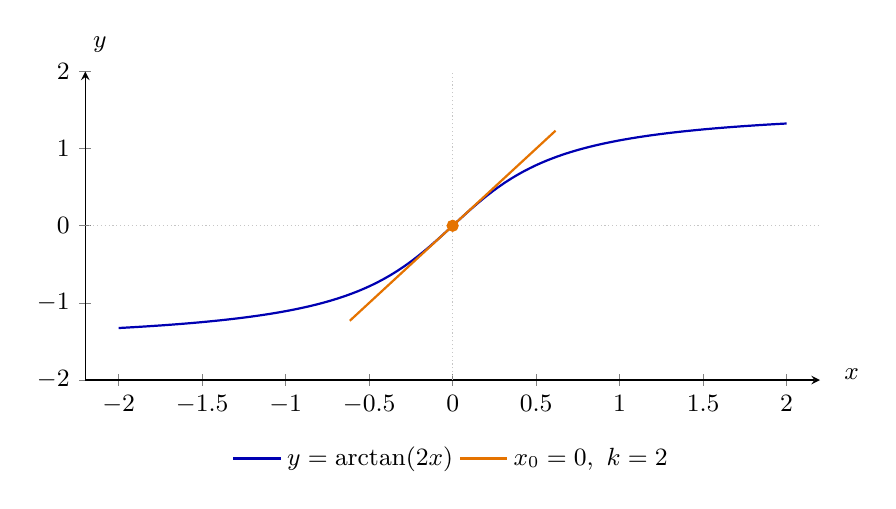
\begin{tikzpicture}[font=\small,>=stealth]
\begin{axis}[width=.90\linewidth,height=5.5cm,xmin=-2.2,xmax=2.2,ymin=-2,ymax=2,
axis lines=left,xlabel={$x$},ylabel={$y$},font=\small,
xlabel style={at={(axis description cs:1.02,.02)},anchor=west},
ylabel style={rotate=-90,at={(axis description cs:.02,1.03)},anchor=south},
legend style={at={(axis description cs:.5,-.18)},anchor=north,draw=none,fill=none,font=\small,legend columns=2},
unbounded coords=jump,clip=true,]
\addplot[gray!45,thin,densely dotted,forget plot] coordinates {(-2.2,0) (2.2,0)};
\addplot[gray!45,thin,densely dotted,forget plot] coordinates {(0,-2) (0,2)};
\addplot[blue!70!black,thick] coordinates {(-2,-1.3258177) (-1.9777778,-1.3231757) (-1.9555556,-1.3204773) (-1.9333333,-1.3177207) (-1.9111111,-1.314904) (-1.8888889,-1.3120254) (-1.8666667,-1.3090828) (-1.8444444,-1.3060741) (-1.8222222,-1.3029971) (-1.8,-1.2998495) (-1.7777778,-1.2966289) (-1.7555556,-1.2933328) (-1.7333333,-1.2899586) (-1.7111111,-1.2865036) (-1.6888889,-1.2829649) (-1.6666667,-1.2793395) (-1.6444444,-1.2756244) (-1.6222222,-1.2718162) (-1.6,-1.2679115) (-1.5777778,-1.2639067) (-1.5555556,-1.259798) (-1.5333333,-1.2555816) (-1.5111111,-1.2512533) (-1.4888889,-1.2468086) (-1.4666667,-1.2422432) (-1.4444444,-1.237552) (-1.4222222,-1.2327302) (-1.4,-1.2277724) (-1.3777778,-1.222673) (-1.3555556,-1.2174261) (-1.3333333,-1.2120257) (-1.3111111,-1.206465) (-1.2888889,-1.2007373) (-1.2666667,-1.1948354) (-1.2444444,-1.1887515) (-1.2222222,-1.1824776) (-1.2,-1.1760052) (-1.1777778,-1.1693253) (-1.1555556,-1.1624283) (-1.1333333,-1.1553042) (-1.1111111,-1.1479424) (-1.0888889,-1.1403316) (-1.0666667,-1.1324598) (-1.0444444,-1.1243144) (-1.0222222,-1.1158821) (-1,-1.1071487) (-0.97777778,-1.0980992) (-0.95555556,-1.0887176) (-0.93333333,-1.0789872) (-0.91111111,-1.0688899) (-0.88888889,-1.0584069) (-0.86666667,-1.047518) (-0.84444444,-1.036202) (-0.82222222,-1.0244363) (-0.8,-1.012197) (-0.77777778,-0.99945885) (-0.75555556,-0.98619507) (-0.73333333,-0.97237743) (-0.71111111,-0.95797612) (-0.68888889,-0.94295973) (-0.66666667,-0.92729522) (-0.64444444,-0.9109479) (-0.62222222,-0.89388147) (-0.6,-0.87605805) (-0.57777778,-0.85743823) (-0.55555556,-0.83798123) (-0.53333333,-0.81764505) (-0.51111111,-0.79638673) (-0.48888889,-0.77416268) (-0.46666667,-0.75092906) (-0.44444444,-0.72664234) (-0.42222222,-0.70125992) (-0.4,-0.67474094) (-0.37777778,-0.64704719) (-0.35555556,-0.61814423) (-0.33333333,-0.5880026) (-0.31111111,-0.55659932) (-0.28888889,-0.52391935) (-0.26666667,-0.48995733) (-0.24444444,-0.45471927) (-0.22222222,-0.41822433) (-0.2,-0.38050638) (-0.17777778,-0.34161549) (-0.15555556,-0.30161905) (-0.13333333,-0.26060239) (-0.11111111,-0.21866895) (-0.088888889,-0.17593963) (-0.066666667,-0.13255153) (-0.044444444,-0.088655882) (-0.022222222,-0.044415215) (0,0) (0.022222222,0.044415215) (0.044444444,0.088655882) (0.066666667,0.13255153) (0.088888889,0.17593963) (0.11111111,0.21866895) (0.13333333,0.26060239) (0.15555556,0.30161905) (0.17777778,0.34161549) (0.2,0.38050638) (0.22222222,0.41822433) (0.24444444,0.45471927) (0.26666667,0.48995733) (0.28888889,0.52391935) (0.31111111,0.55659932) (0.33333333,0.5880026) (0.35555556,0.61814423) (0.37777778,0.64704719) (0.4,0.67474094) (0.42222222,0.70125992) (0.44444444,0.72664234) (0.46666667,0.75092906) (0.48888889,0.77416268) (0.51111111,0.79638673) (0.53333333,0.81764505) (0.55555556,0.83798123) (0.57777778,0.85743823) (0.6,0.87605805) (0.62222222,0.89388147) (0.64444444,0.9109479) (0.66666667,0.92729522) (0.68888889,0.94295973) (0.71111111,0.95797612) (0.73333333,0.97237743) (0.75555556,0.98619507) (0.77777778,0.99945885) (0.8,1.012197) (0.82222222,1.0244363) (0.84444444,1.036202) (0.86666667,1.047518) (0.88888889,1.0584069) (0.91111111,1.0688899) (0.93333333,1.0789872) (0.95555556,1.0887176) (0.97777778,1.0980992) (1,1.1071487) (1.0222222,1.1158821) (1.0444444,1.1243144) (1.0666667,1.1324598) (1.0888889,1.1403316) (1.1111111,1.1479424) (1.1333333,1.1553042) (1.1555556,1.1624283) (1.1777778,1.1693253) (1.2,1.1760052) (1.2222222,1.1824776) (1.2444444,1.1887515) (1.2666667,1.1948354) (1.2888889,1.2007373) (1.3111111,1.206465) (1.3333333,1.2120257) (1.3555556,1.2174261) (1.3777778,1.222673) (1.4,1.2277724) (1.4222222,1.2327302) (1.4444444,1.237552) (1.4666667,1.2422432) (1.4888889,1.2468086) (1.5111111,1.2512533) (1.5333333,1.2555816) (1.5555556,1.259798) (1.5777778,1.2639067) (1.6,1.2679115) (1.6222222,1.2718162) (1.6444444,1.2756244) (1.6666667,1.2793395) (1.6888889,1.2829649) (1.7111111,1.2865036) (1.7333333,1.2899586) (1.7555556,1.2933328) (1.7777778,1.2966289) (1.8,1.2998495) (1.8222222,1.3029971) (1.8444444,1.3060741) (1.8666667,1.3090828) (1.8888889,1.3120254) (1.9111111,1.314904) (1.9333333,1.3177207) (1.9555556,1.3204773) (1.9777778,1.3231757) (2,1.3258177)};
\addlegendentry{$y=\arctan(2x)$}
\addplot[orange!90!black,thick] coordinates {(-0.616,-1.232) (0.616,1.232)};
\addlegendentry{$x_0=0,\ k=2$}
\addplot[only marks,mark=*,orange!90!black,forget plot] coordinates {(0,0)};

\end{axis}
\end{tikzpicture}
\par\smallskip{\small 按本题原函数绘图；切线斜率由本题的导函数计算。}
\end{center}


\end{minipage}
令 $u=2x$，$u'=2$，得
\[
y'=\frac{2}{1+4x^2},\qquad y'(0)=2,\quad y(0)=0.
\]
切线方程为 $y=2x$。这是复合求导的拓展示例，不要求高考直接记忆反三角公式。
\end{examplebox}

